% --------------------------------------------------------------------
% Preamble
% --------------------------------------------------------------------
\documentclass[a4paper]{article}	

\usepackage[scaled]{helvet}
\renewcommand\familydefault{\sfdefault} 
\usepackage[T1]{fontenc}

% 'microtype' can only be used with pdflatex
\usepackage[protrusion=true,expansion=true]{microtype}

	
\usepackage[utf8]{inputenc}
\usepackage[english]{babel}
\usepackage{amsmath,amsfonts,amsthm,amssymb}
\usepackage{stix}
\usepackage{graphicx}
\usepackage{xcolor}

% Spacing between lines 
\usepackage{setspace}
\onehalfspacing

% ----- page layout 
\usepackage[
	a4paper,
	top=1in, bottom=1.25in, left=1.25in, right=1.25in
]{geometry}	

\setlength{\oddsidemargin}{5mm}			% Remove 'twosided' indentation
\setlength{\evensidemargin}{5mm}

% ----- To allow cross-referencing between documents
%       a common root folder must be established
%       this command encapsulates the path
\newcommand{\qmPath}{../quality_manual_document}%

% ------ To cross reference other documents, works with hyperref
\usepackage{xr-hyper}

% ------ External references used in this manual
\externaldocument[GRP-]{../guidelines_reporting_publishing/MSL_Guidelines_Reporting_Publishing}

\usepackage[
	colorlinks=true,
	urlcolor=magenta,
	linkcolor=blue, 	% [red]
%	anchorcolor 	 % [black]
	citecolor=blue, 		% [green]
	filecolor=cyan, 	% [cyan]
	menucolor=black		% [red]
]{hyperref}

% Header and footer control
\usepackage{fancyhdr}
\setlength{\headheight}{15.2pt}
\pagestyle{fancy}

% ----- Table of contents 
\usepackage{titletoc}
\usepackage{tocloft}

\renewcommand\cftsecfont{\normalfont}
\renewcommand\cftsecpagefont{\normalfont}
\renewcommand{\cftsecleader}{\cftdotfill{\cftsecdotsep}}
\renewcommand\cftsecdotsep{\cftdot}
\renewcommand\cftsubsecdotsep{\cftdot}

% ----- Tables
\usepackage{booktabs}
\usepackage{colortbl}
\usepackage{longtable}
\usepackage{makecell}

% ----- Units formatting 
\usepackage{siunitx}

% ------ Macros for this document
\definecolor{yellowMSL}{RGB}{244,182,8}

% Mark-up for small changes (a few words only)
\newcommand{\proposed}[1]{{\color{cyan}{{#1}}}}
\newcommand{\deprecated}[1]{{\color{yellowMSL}{#1}}}

% Mark-up for paragraphs. 
\usepackage{framed}
\newcommand{\proposedbox}[1]{
\colorlet{shadecolor}{gray!10}
{\color{cyan}\begin{shaded}
	{#1}
\end{shaded}}
}%

\newcommand{\deprecatedbox}[1]{
\colorlet{shadecolor}{gray!10}
{\color{yellowMSL}\begin{shaded}
	{#1}
\end{shaded}}
}%

% --------------------------------------------------------------------
% Front page definitions (do not change this)
% --------------------------------------------------------------------
\newcommand{\HRule}[1]{\rule{\linewidth}{#1}} 	% Horizontal rule

\makeatletter							% Title
\def\printtitle{%						
    {\centering \@title\par}}
\makeatother									

\makeatletter							% Author
\def\printauthor{%					
    {\raggedright \Large \@author}}				
\makeatother							


% --------------------------------------------------------------------
% Details of what to put on the front page (Change this)
% --------------------------------------------------------------------
\title{	\Large 
	\textsc{ Measurement Standards Laboratory of New Zealand } \\ [2.0cm]			
	\HRule{2pt} \\ [0.25cm]						
	\LARGE \textbf{\uppercase{Quality Manual}}	% Title
	\HRule{2pt} \\ [0.25cm]		
	\Large \today			
}

\author{
Measurement Quality Council\\	
Measurement Standards Laboratory of New Zealand\\	
}

\begin{document}
\hypersetup{pageanchor=false}	% prevents a warning message
\fancyhf{}	% Header and footer are empty

% ------------------------------------------------------------------------------
% Title page
% ------------------------------------------------------------------------------
\thispagestyle{empty}		% Remove page numbering on this page
\pagestyle{plain}			% puts pages numbers back in front matter

\printtitle					% Print the title data as defined above
  	\vfill
\printauthor				% Print the author data as defined above
\newpage

\pagenumbering{roman}

\tableofcontents
\newpage

% ----- Place the signed Quality Policy Statement prominently 
\addcontentsline{toc}{section}{Quality policy statement}
\section*{Quality policy statement}
\label{ss:quality_policy_statement}
This signed statement is stored in the central files system. 

\begin{center}

\includegraphics[width=1.05\textwidth]{pictures/MSL_qps_(signed)}
\end{center}
\clearpage


% ----- Main document now begins
\pagestyle{fancy}			% Turn on footer style control
\pagenumbering{arabic}
\hypersetup{pageanchor=true}
\setcounter{page}{1}		% Set page numbering to begin on this page
\fancyfoot[L]{MSL Quality Manual}
\fancyfoot[C]{\today}
\fancyfoot[R]{Page \thepage\ of \pageref*{LastPage}}

\setlength{\parindent}{0cm}	% No indent when starting a new paragraph
\setlength{\parskip}{\baselineskip}	% Leave a blank line between paragraphs

% ----- These files contain the document content
\section{Introduction}
The Measurement Standards Laboratory of New Zealand (MSL) is New Zealand's National Measurement Institute (NMI). MSL is designated as the verifying authority of New Zealand's national measurement standards by act of parliament. All results quoted in measurement, calibration and test reports issued by MSL are directly traceable to the national measurement standards held by the laboratory. 

New Zealand is a signatory to the international Meter Convention \cite{Metre_convention}, which establishes a world-wide system of measurement units. 
MSL plays a key role in ensuring international recognition of New Zealand's measurement system. 

MSL is a signatory of an international Mutual Recognition Agreement (MRA) \cite{MRA_1999} that provides a framework for NMIs to demonstrate the performance of measurement capabilities that support calibration and measurement services. One of the MRA requirements for mutual recognition is that each NMI implement a suitable system for ensuring quality. MSL has implemented a quality management system (QMS) that is accredited, by International Accreditation New Zealand (IANZ), against the ISO 17025 standard for testing and calibration laboratories \cite{ISO_17025}. 

For the purpose of accreditation against ISO/IEC 17025, the scope of the QMS covers all MSL activities that relate to the provision of traceable calibration and measurement services within MSL's scope of accreditation.  This includes realisation and maintenance of standards, calibration, and product testing. 

This Quality Manual also covers activities that are related to MSL's role as an NMI but are not part of ISO 17025.  Such activities include research, training and dissemination and consultancy.\clearpage
\section{Organisational structure}
\label{s:organisation}
MSL operates as a group within Callaghan Innovation. The structure of Callaghan Innovation and the structure of MSL are summarised below.

\subsection{Callaghan Innovation}
Callaghan Innovation is a Crown Agent of the New Zealand government. 

\deprecated{Callaghan Innovation is led by a Chief Executive Officer and divided into a number of Hap\=u, each managed by a Chief reporting to the Chief Executive. Innovation Expertise is one of these Hap\=u, within which MSL is a Hap\=u team. A Director manages MSL.}

\deprecated{Inside the MSL group, the role of Team Manager is recognised as someone who reports to the MSL Director and supervises staff.} 

Callaghan Innovation also maintains a register of designated Work Area Managers. The role of Work Area Manager is important to the organisation in meeting statutory Health and Safety requirements. 
Work Area Managers report on Health and Safety issues to their respective Group Managers.

\subsection{Measurement Standards Laboratory}
MSL identifies the following roles:
\begin{itemize}
\item	Director
\item	Chief Metrologist
\item	Quality Manager
\item	Team Manager
\item	Member
\item	Quality Council Member
\end{itemize}
The appointment of staff in relation to MSL's role as New Zealand's National Metrology Institute (NMI) is described in section 2.2.3 below.
\subsubsection{Responsibilities} 
\begin{itemize}
\item	All staff in the MSL group at Callaghan Innovation and any other individuals authorised to carry out test and calibration work (i.e., individuals named in the Technical Competency Matrix) operate under the terms of this Quality Manual.
\item	The Chief Metrologist acts as a verifying authority in relation to the verification of any standard or standards of measurement in New Zealand.  The role of the Chief Metrologist shall be given to the Quality Manager or to another MSL Member.  
\item	The role of Director is of particular relevance to the Metre Convention. The Director also makes the necessary delegations to implement the QMS. The MSL Group Manager is currently the Director of MSL. 
\item	The Quality Manager ensures that the QMS is implemented and followed, oversees the management and improvement of the QMS and ensures that MSL's scope of accreditation, and its Calibration and Measurement Capabilities (CMCs) in Appendix C of the MRA, are 
consistent with each other.
\item	Members of the Quality Council (MQC) maintain the QMS, and the Quality Manual.

\end{itemize}

\paragraph{Impartiality}
\label{sssp:impartiality}
All staff shall act impartially.

Teams shall be responsible for identifying and documenting potential risks to impartiality. Team managers will take account of these records when assigning tasks to staff.

Potential risks to impartiality may be identified by the process described in the corporate document \deprecated{``Declaring Interests and Managing Conflict Policy.docx''}. Individuals' declarations will not be available to other staff, but team Managers will have access to this information and can manage the associated risks. The accreditation body will not be able to access this private information. 

The Risks and Opportunities register will be used to record potential risks to impartiality that are not subject to privacy constraints. The Risks and Opportunities register is part of the central file system (~see~\ref{ss:central_file_system}~).

\paragraph{The Quality Manager}
A Quality Manager is required by ISO 17025. 

Although the title Quality Manager need not be used, someone must be 
assigned the Quality Manager functions. 

A senior metrologist is usually appointed as Quality Manager. So, that person occupies a line management position under the \deprecated{MSL Director} and Team managers. This should not present a problem provided that, on matters of quality, the Quality Manager has direct access to the highest level of management in the organisation at which policy and resourcing decisions are made affecting the 
laboratory.

The Quality Manager is responsible for implementing and operating the quality system on a day-to-day basis. He or she is normally responsible for administering the quality management system, for compiling the quality manual and for organising reviews and audits of the quality system.

While the role has a large administrative component, the Quality Manager is ultimately responsible for effective enforcement of quality policy. 

The Quality Manager is distinct from \deprecated{the MSL Director and Team manager roles}. The responsibility is discharged through monitoring and advising not by managing technical activities directly.

The Quality Manager will advise management on quality issues and also has a responsibility to report to the APMP Technical Committee on Quality Systems on matters of quality relating to MSL.
The Quality Manager role requires familiarity with ISO 17025 and knowledge of the MSL quality system. Suitable experience could be acquired, for example, by acting as an IANZ Technical Expert to assess commercial calibration laboratories, and by serving on the MSL Quality Council.

\subsubsection{MSL Sections}
MSL is organised into three technical teams, each comprised of sections aligned with different technical areas of the SI (~see figure~\ref{fig:org_msl}~).

The sections are: 
\begin{itemize}
\item	Length
\item	Time and Frequency 
\item	Electrical 
\item	Temperature and Humidity
\item	Photometry and Radiometry
\item	Mass and Pressure
\end{itemize}

Sections are involved in:
\begin{itemize}
\item	maintenance and development of measurement standards; 
\item	calibration and measurement services;
\item	scientific research;
\item	liaison with international metrology groups and networks of peers; 
\item	dissemination of knowledge and technical services within New Zealand.
\end{itemize}

Third-party accreditation of MSL by IANZ is organised by section, and sometimes by sub-section (e.g., Pressure, Mass and related quantities, Temperature, and Humidity are typically treated as distinct disciplines for technical reviews).

\begin{figure}
\begin{center}
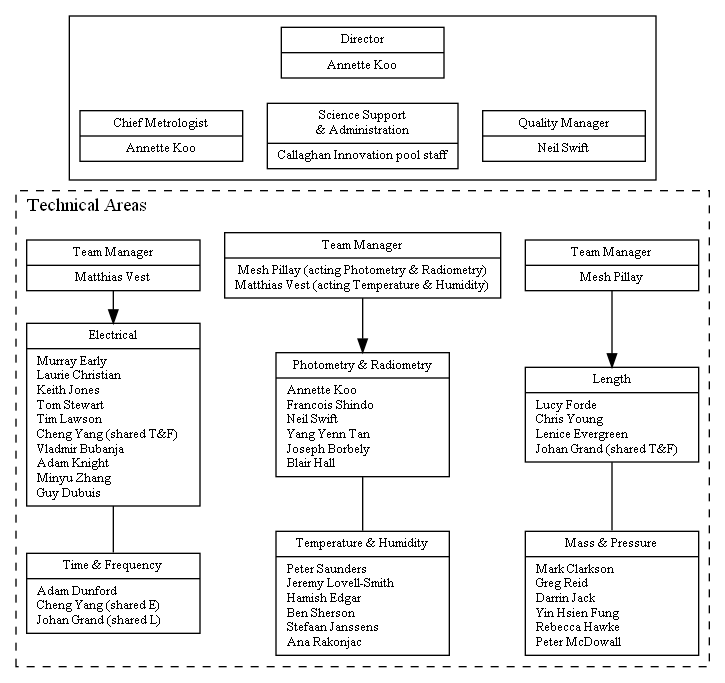
\includegraphics[width=1.1\textwidth]{pictures/MSL_org_full}
\end{center}
\caption{MSL Organisational Structure (September 2, 2022)}
\label{fig:org_msl}
\end{figure}


\subsubsection{Approvals}
\paragraph{Chief Metrologist}    

The appointment of the Chief Metrologist in relation to MSL's role as the New Zealand NMI is done in the context of the Measurement Standards Act 1992 \cite{MS_ACT_1992} and the National Standards Regulations 2019 \cite{NS_Regulations}.
The National Standards Regulations 2019 (as at 20 May 2019) has the definition:
\begin{quote}
Measurement Standards Laboratory of New Zealand means the laboratory of Callaghan 
Innovation (established under section 7 of the Callaghan Innovation Act 2012) that maintains 
the principal standard measures for New Zealand.
\end{quote}
This is interpreted as being the responsibility of Callaghan Innovation to define (effectively delegated from the Minister, through the regulation). Under this interpretation, the Chief Executive Officer shall appoint, in writing, the Chief Metrologist. The Chief Metrologist shall be a senior metrologist with knowledge of and familiarity with the New Zealand and international measurement infrastructure. The roles of Director and Chief Metrologist may be combined.
Under the National Standards Regulations, the Chief Metrologist may delegate, in writing, to any other person who is an MSL Member.
\paragraph{Team Manager}
Technical activities are organised into three teams, each with a manger who has overall responsibility for technical operations, including provision of the resources needed to ensure the required quality of laboratory operations. 
\paragraph{Quality Manager}
The Director appoints the Quality Manager. Appointments are for a period of two years, which may be extended. 

The Quality Manager has the responsibility and authority to ensure that the quality management system is implemented and adhered to at all times; the Quality Manager has direct access to the highest levels of management at which decisions are made on laboratory policy or resources (\deprecated{currently the Chief of Innovation Expertise}).

The Quality Manager may delegate, in writing, to any MSL Member.

When the Quality Manager is absent, the Chief Metrologist automatically assumes the relevant responsibilities.  The Chief Metrologist may re-delegate such responsibilities. 
%
\paragraph{Member}
Members are qualified for particular roles in relation to specific technical procedures. Members are listed in the Technical Competency Matrix (TCM, the TCM is part of the central files system described in section 4.2 ). Note, some individuals in the TCM may be under contract to MSL or be employees of Callaghan Innovation outside MSL. 

An MSL Member who has been approved as a signatory by IANZ for particular items in the scope of accreditation is authorised to sign IANZ endorsed certificates and reports for these items.

%\deprecated{Note that in clause 8(2)(a) of the National Standards Regulations 1976 (as at 1 May 2014), with Amendment No.1 (1992), which relates to delegation of the powers of a verifying authority, the reference to 'any other person who works in that laboratory;' is interpreted as an MSL Member. }

{Note that in clause 8(2)(a) of the National Standards Regulations 2019, in relation to delegation of the power of a verifying authority, the reference to 'a person working in the Measurement Standards Laboratory of New Zealand' is interpreted as an MSL Member.}

\paragraph{Quality Council}
After consultation with the Director, the Quality Manager appoints, in writing, the members of the MSL Quality Council (MQC). Membership tends to be for periods of several months, so that representation can be shared across MSL over time.

\paragraph{Leadership Team}
The MSL Leadership Team includes the Director, the Chief Metrologist, the Quality Manager, the 
Team Managers and the Science Support Coordinator. 

\subsubsection{MSL Affiliations}
\label{sss:affiliations}
\begin{itemize}

\item	MSL is accredited, by IANZ, as an accredited Metrology and Calibration Laboratory complying with NZS/ISO/IEC 17025 (original date of accreditation, 30 July 2004). 

\item	The Chief Metrologist is authorised by the Minister of Science and Innovation, under the Measurement Standards Regulations, 
%\deprecated{1976, Amendment 1}%
to act as a verifying authority in relation to the verification of any standard or standards of measurement in New Zealand.

\item	New Zealand is a signatory to the Metric Treaty of 1875 and hence is a member state of the Metre Convention.  New Zealand (through the Ministry of Business, Innovation and Employment) subscribes annually to the Comit\'e International des Poids et Mesures (CIPM) which administers the Metre Convention, provides technical coordination, and is the owner of the Syst\`eme International d'Unit\'es (SI). The Ministry of Business, Innovation and Employment handles the administrative aspects of New Zealand relationship with the CIPM, 
while MSL handles the technical aspects, and provides a New Zealand representative (normally the MSL Director) to the Conf\'erence G\'en\'erale des Poids et Mesures (CGPM).

\item	MSL is a signatory to the Mutual Recognition Arrangement on National Measurement Standards and Calibration Measurement Certificates Issued by National Metrology Institutes (MRA) drawn up by the CIPM under the authority given to it under the Metric Treaty.

\item	MSL is a permanent member of four of the Consultative Committees (CCs) that assist the BIPM with its scientific work: CCT (Thermometry), CCEM (Electricity and Magnetism), CCPR (Photometry and Radiometry) and CCM (Mass and related units). 

\item	MSL and IANZ have signed a Memorandum of Understanding (MOU) formalising the relationship between the national metrology institute and the national laboratory registration agency, as required for recognition by the European Union (EU), of New Zealand testing and certification. The Measurement and Calibration Professional Advisory Committee, chaired by the Chief Metrologist, provides the vehicle for operating the MOU.

\item	MSL and the National Measurement Institute, Australia (NMIA), have signed seven agreements recognising the equivalence of the following units: metre, kilogram, volt, ohm, farad, second, kelvin.

\item	MSL is a full member of the Asia-Pacific Metrology Programme (APMP). This Regional Metrology Organisation (RMO) is a member of the Joint Committee of Regional Metrology Bodies and the BIPM (JCRB) that plays a key role in operating the MRA.
\end{itemize} 
\clearpage
\section{Quality Assurance}

\subsection{Policy on the Quality Assurance of Measurement Capabilities}
\label{ss:quality_assurance_policy}
MSL sections will monitor the performance of all measurement capabilities. 

Monitoring must be planned and will include both internal and external activities. 

The results of quality assurance activities will be continuously reviewed within the section so that appropriate action can be taken to prevent unsatisfactory measurement capabilities from being used. 

Any results that suggest the performance of a measurement capability is inferior to the current accredited scope must be documented and investigated by the section. The MQC must be notified immediately about any discrepant results. The MQC will maintain a record of such instances, including a report about the corrective actions taken. 

Internal quality assurance activities shall be used to monitor the performance of measurement procedures. For example, 
\begin{itemize}
\item	regular use of certified reference materials and/or reference material and/or quality control 
material;

\item	regular use of alternative metrologically traceable instrumentation;

\item	functional checks of measuring and testing equipment;

\item	use of check-standards with control charts and/or control limits;

\item	periodic intermediate checks on measuring equipment;

\item	replicate tests or calibrations using the same or different methods;

\item	re-testing or recalibration of retained items; inter-operator comparisons;    
\end{itemize}

External quality assurance activities within the accredited scope should be planned, if possible, to occur over the usual accreditation cycle. These activities generally involve participation in international measurement comparisons with other NMIs.     

A central register of all MSL participation in international comparisons will be maintained in the QMS and will include a copy of comparison reports, which will be reviewed.  




%MSL Quality Policy Statement
%The Measurement Standards Laboratory (MSL) is New Zealand's National Metrology Institute (NMI). 
%MSL is responsible for developing and disseminating the physical measurement standards needed in 
%New Zealand and ensuring that they are accepted nationally and internationally. MSL's activities 
%support measurement capabilities that underpin New Zealand's prosperity and quality of life. 
%We aim to provide the services that our customers need and, through a process of continuous 
%improvement, to anticipate those needs and exceed our customers' expectations. We are 
%committed to providing a quality service in a safe and healthy working environment. 
%MSL's calibration and testing services are accredited by International Accreditation New Zealand 
%(IANZ), against the ISO 17025 standard for testing and calibration laboratories, using internationally 
%recognised technical experts in each area. The capability of these services is documented in the MSL 
%Scope of Accreditation schedule issued by IANZ. 
%As an NMI, MSL: 
%*	participates in international activities that ensure mutual recognition of New Zealand's and 
%other nations measurement capabilities; 
%*	provides technical measurement services for the public and private sectors; 
%*	engages in research and development activities that support the scientific and technical 
%foundation of the international measurement system; 
%*	provides scientific leadership to New Zealand's National Quality Infrastructure in the form of 
%authoritative and independent scientific advice on measurement; 
%*	provides knowledge transfer and advice for industry, Government and academia.
%MSL is committed to the level of quality expected from a national centre of excellence in metrology. 
%MSL management and staff are committed to complying with ISO 17025 and to seeking continual 
%improvement in the effectiveness of the management system. MSL staff and individuals qualified to 
%carry out test and calibration activities adhere to the policies and procedures documented in the 
%quality management system. 
%The quality of services and other activities are monitored and regularly reviewed, using information 
%collected from:
%*	client satisfaction surveys and customer feedback;
%*	MSL's performance in international measurement comparisons;
%*	international peer-reviews of calibration and measurement services;
%*	management reviews of the Quality Management System;
%*	IANZ audits of the Quality Management System;
%*	MSL audits of calibration and measurement services and the Quality Management System;
%*	MSL reviews of technical areas;
%*	health and safety audits of work areas. 


\clearpage
\input{\qmPath/Document_control}\clearpage
\input{\qmPath/Competencies_and_training}\clearpage
\input{\qmPath/Reporting_and_publishing}\clearpage
\input{\qmPath/Goods_control}\clearpage
\input{\qmPath/Audits_and_reviews}\clearpage
\input{\qmPath/Requests_and_contracts}\clearpage
\input{\qmPath/Improvements}\clearpage
\input{\qmPath/Project_management}\clearpage

\appendix	% Changes the style of the headings for sections
\input{\qmPath/Abbreviations}\clearpage
\input{\qmPath/Calendar}\clearpage
\input{\qmPath/Cross_reference_17025}\clearpage

% ----- Label for the very last page, so that we can do "page x of N"
\input{../quality_manual_document/References}	% Don't create a blank last page 
\label{LastPage}~

\end{document}